
\begin{frame}[fragile]{Module cảm biến đeo: Luồng làm việc}
    \begin{columns}[t]
        \begin{column}{0.6\textwidth}
            \begin{figure}
                \centering
                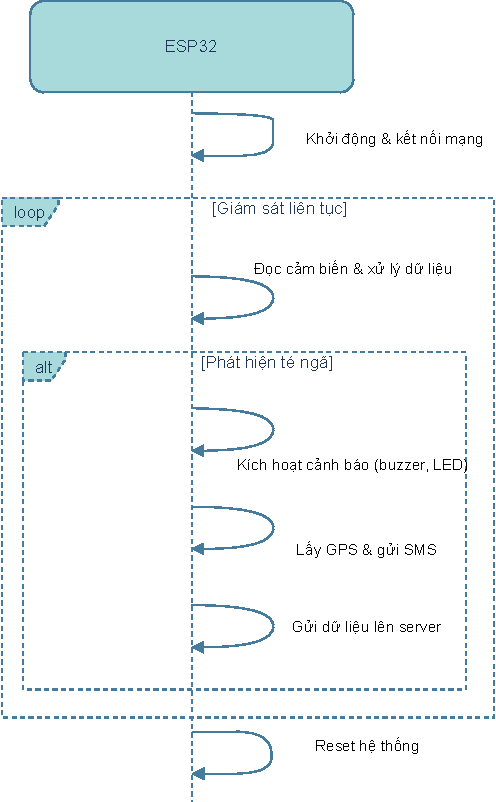
\includegraphics[width=0.85\textwidth,height=0.6\textheight,keepaspectratio]{images/module1_time_flow.pdf}
            \end{figure}
        \end{column}
        \begin{column}{0.4\textwidth}
            \begin{block}{Quy trình}
                \begin{itemize}
                    \item Điều phối từ thu thập dữ liệu cảm biến đến xử lý sự kiện và kích hoạt cảnh báo.
                    \item Minh họa luồng làm việc:
                \end{itemize}
            \end{block}
            \begin{block}{Mô tả}
                \begin{itemize}
                    \item Lưu đồ luồng làm việc của mô-đun phát hiện té ngã trên ESP32.
                \end{itemize}
            \end{block}
            \label{fig:module1_flow}
        \end{column}
    \end{columns}
\end{frame}

% Slide: Tổng quan mô-đun nhúng (OK - không cần sửa)
\begin{frame}{Module cảm biến đeo: Tổng quan mô-đun nhúng}
    \begin{block}{Tổng quan}
        \begin{itemize}
            \item Triển khai trên vi điều khiển \textbf{ESP32}: nút cảm biến và trung tâm cảnh báo.
            \item Chức năng chính:
            \begin{itemize}
                \item Thu thập dữ liệu chuyển động từ cảm biến.
                \item Phân tích thuật toán phát hiện té ngã.
                \item Cảnh báo thời gian thực: cục bộ (buzzer, LED) và từ xa (Wi-Fi/4G, MQTT, SMS).
            \end{itemize}
        \end{itemize}
    \end{block}
\end{frame}

% Slide: Môi trường phát triển 
\begin{frame}{Module cảm biến đeo: Môi trường phát triển}
    \begin{block}{Chi tiết}
        \begin{itemize}
            \item Phần mềm xây dựng trên \textbf{ESP-IDF} (Espressif IoT Development Framework).
            \item Hệ thống build: \textbf{CMake}, quản lý qua \texttt{idf\_component.yml}.
            \item API: UART, I2C, SPI, PWM, GPIO, Wi-Fi, MQTT, HTTP.
            \item Cấu hình qua \textbf{Kconfig}, lưu trong \texttt{sdkconfig}.
            \item Đảm bảo ổn định, mở rộng, tương thích driver.
        \end{itemize}
    \end{block}
\end{frame}

% Slide: Cấu trúc phần mềm
\begin{frame}[fragile]{Module cảm biến đeo: Cấu trúc project}
    \renewcommand{\baselinestretch}{0.8}
    \begin{minted}[fontsize=\scriptsize, breaklines, bgcolor=lightgray]{text}
mainproject/
├── main/
│   ├── main.c
│   ├── app_main.c
│   └── app_main.h
├── components/
│   ├── buzzer/
│   ├── comm/
│   ├── data_manager/
│   ├── event_handler/
│   ├── fall_logic/
│   ├── json_wrapper/
│   ├── led_indicator/
│   ├── mpu6050/
│   ├── sim4g_gps/
│   ├── user_mqtt/
│   └── wifi_connect/
    \end{minted}
    \renewcommand{\baselinestretch}{1.0}
\end{frame}

% Slide: Mô tả các thành phần (SỬA LẠI - tách thành 2 slide nếu cần)
\begin{frame}{Module cảm biến đeo: Mô tả các thành phần}
    \begin{columns}[t]
        \begin{column}{0.48\textwidth}
            \begin{block}{Thành phần chính}
                \begin{itemize}
                    \item \textbf{main.c}: Gọi \texttt{app\_main()}.
                    \item \textbf{app\_main.c/h}: Điều phối, khởi tạo.
                    \item \textbf{fall\_logic}: Thuật toán phát hiện té ngã.
                    \item \textbf{event\_handler}: Phản ứng sự kiện.
                    \item \textbf{mpu6050}: Driver cảm biến.
                \end{itemize}
            \end{block}
        \end{column}
        \begin{column}{0.48\textwidth}
            \begin{block}{Thành phần khác}
                \begin{itemize}
                    \item \textbf{buzzer, led\_indicator}: Cảnh báo cục bộ.
                    \item \textbf{sim4g\_gps, wifi\_connect}: Kết nối từ xa.
                    \item \textbf{user\_mqtt}: Giao tiếp MQTT.
                    \item \textbf{comm, data\_manager}: Quản lý giao tiếp.
                \end{itemize}
            \end{block}
        \end{column}
    \end{columns}
\end{frame}

% Slide: Sơ đồ khối phần mềm (OK - nhưng có thể điều chỉnh height nếu cần)
\begin{frame}[fragile]{Module cảm biến đeo: Sơ đồ khối phần mềm}
    \begin{figure}
        \centering
        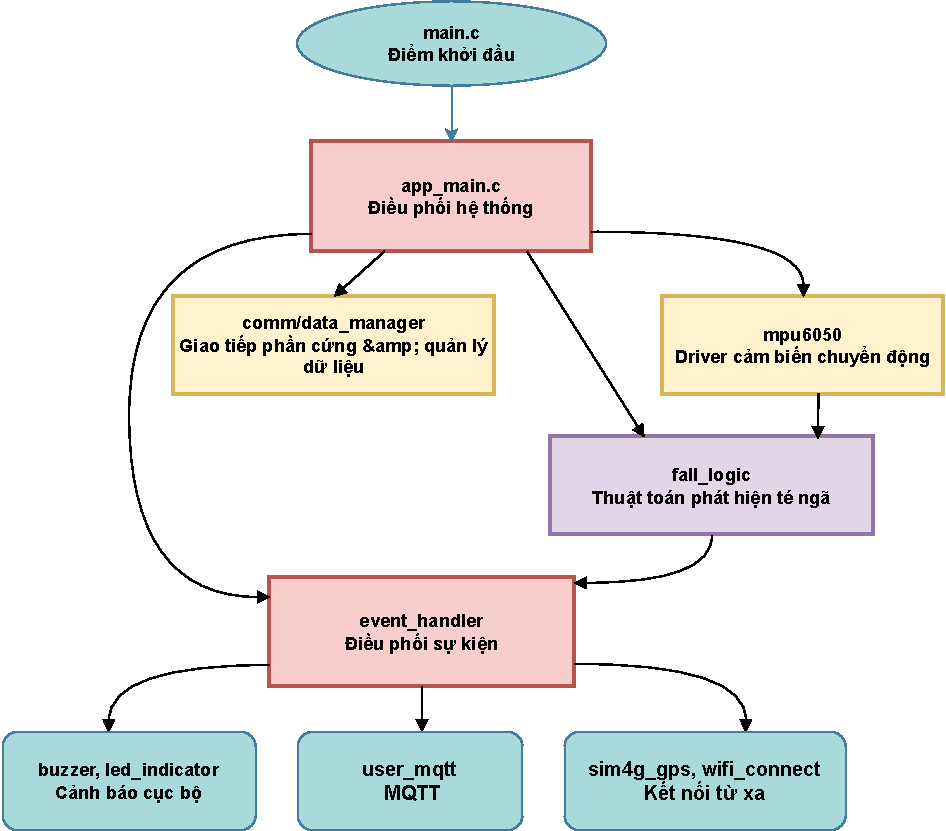
\includegraphics[width=0.85\textwidth,height=0.7\textheight,keepaspectratio]{images/module1_software_block-crop.pdf}
        \caption{Sơ đồ khối phần mềm của mô-đun nhúng ESP32.}
        \label{fig:module1_software_block}
    \end{figure}
\end{frame}

% Slide: Thuật toán phát hiện té ngã
\begin{frame}{Module cảm biến đeo: Thuật toán phát hiện té ngã}
    \begin{block}{Cơ chế}
        \begin{itemize}
            \item Dựa trên \textbf{gia tốc tổng hợp}: 
            \[
            a_{total} = \sqrt{a_x^2 + a_y^2 + a_z^2}
            \]
            \item $a_{total} < \texttt{FALL\_THRESHOLD}$: Đánh dấu sự kiện té ngã.
            \item Ngưỡng điều chỉnh qua \texttt{CONFIG\_FALL\_LOGIC\_THRESHOLD\_G}.
            \item Chạy trong \textbf{tác vụ FreeRTOS}, chu kỳ \texttt{CHECK\_INTERVAL\_MS}.
        \end{itemize}
    \end{block}
    \begin{enumerate}
        \item Đọc dữ liệu từ \texttt{mpu6050}.
        \item Tính gia tốc tổng hợp, so sánh ngưỡng.
        \item Gửi \texttt{EVENT\_FALL\_DETECTED} tới \texttt{event\_handler}.
        \item Đặt cờ \texttt{s\_fall\_detected}, reset qua \texttt{fall\_logic\_reset\_fall\_status()}.
    \end{enumerate}
\end{frame}

% Slide: Lưu đồ thuật toán (OK - nhưng có thể điều chỉnh height)
\begin{frame}[fragile]{Module cảm biến đeo: Lưu đồ thuật toán component fall\_logic}
    \begin{figure}
        \centering
        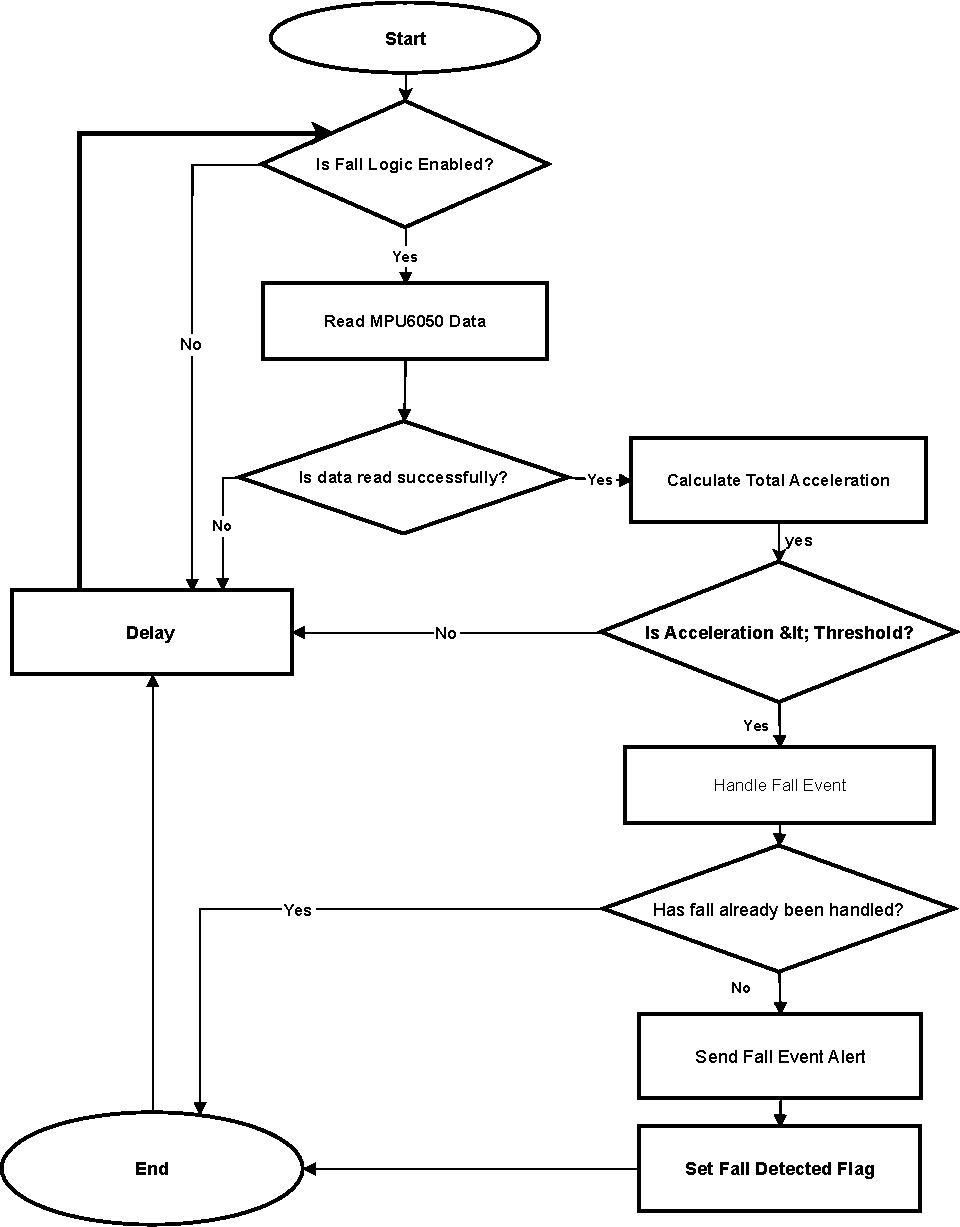
\includegraphics[width=0.85\textwidth,height=0.7\textheight,keepaspectratio]{images/module1_fall_logic_diagram.pdf}
        \caption{Lưu đồ thuật toán phát hiện té ngã.}
        \label{fig:fall_logic_flow}
    \end{figure}
\end{frame}
